%%%%%%%%%%%%%%%%%%%%%%%%%%%%%%%%%%%%%%%%%%%%%%%%%
%%%%%%%%%%%% cap: intro %%%%%%%%%%%%%%%%%
%%%%%%%%%%%%%%%%%%%%%%%%%%%%%%%%%%%%%%%%%%%%%%%%%

\chapter{Introduction}\label{cap:intro}



%%%%%%%%%%%%%%%%%%%%%%%%%%%%%%%%%%%%%%%%%%%%%
%%%%%%%%%%%% Section: Motivation %%%%%%%%%%%%
%%%%%%%%%%%%%%%%%%%%%%%%%%%%%%%%%%%%%%%%%%%%%
\section{Project Motivation}\label{sect:motivation}
\hspace{\parindent} This project started from a wish to create a platform to store all BCI applications developed by the University's(UVT) BCI teams during hackathons and other contests. Being part of said teams, it became apparent that most aforementioned applications could not be operated by a non-abled person.

\vspace*{2mm}
\hspace{\parindent} There are numerous applications developed for BCI systems, with some citing them as being the future of entertainment and the next step, beyond AR and VR for an able-bodied user\cite{future_of_metaverse_BCI}. That leaves a lot to be desired when it comes to the initial purpose of the BCI, which was to be a prosthetic for the brain. The research for BCI came a long way since early experimentation on primates in the late 60s {\bfseries(CITATION DAVE)}, with modern BCIs being used for both medical purposes and entertainment. However, there appears to be a lack of consumer solutions when it comes to housing multiple applications in one place.

{\bfseries(TODO: MORE EXPLANATIONS NEEDED)}

\vspace*{2mm}
\hspace{\parindent} There are numerous applications being developed for BCI users. The applications are however disconnected from one another such as the end-users would have a hard time adjusting from one to the other on their own. This is a major problem, since the end-user is more often than not a disabled person requiring a a helper. I wanted to create an application that would solve this issue, something that would allow a disabled user the freedom to open different apps and close them at his/her own leisure with minimal help. I chose this topic of this bachelor's thesis in the hopes of creating such an app and in the hopes of making it easier for a disabled person to do the thing I loved doing all my life: use a computer.



%%%%%%%%%%%%%%%%%%%%%%%%%%%%%%%%%%%%%%%%%%%%%
%%%%%%%%%%%% Section: Objectives %%%%%%%%%%%%
%%%%%%%%%%%%%%%%%%%%%%%%%%%%%%%%%%%%%%%%%%%%%
\section{Objectives}\label{sect:objectives}
\hspace{\parindent} From a general standpoint, the main objective of the platform is described in the above section of this paper: making a cohesive application that integrates with a well-known BCI speller to deliver seamless access to different apps for a disabled user. The platform should be intuitive and easy to use, such as no explanations should be needed before using the platform. 

\vspace*{2mm}
\hspace{\parindent} From a technical standpoint, the objective of this project is to create a stable system capable of housing a considerable quantity of applications without failure. Due to the platform relying on multiple components (the speller, the individual applications, the speller receiver, the platform logic itself), multiple points of failure exist. In the case of an unhandled crash, an able-bodied helper is once again needed, thus defeating the general purpose of the app. As such, error handling inside the application is prioritary. 

\vspace*{2mm}
\hspace{\parindent} When it comes to compatibility, the objective is making apps integrate with the platform. This requires modyfing the apps to be contained inside the platform so as to make them compatible. To reach this objective without compromising the aforementioned two, the platform will require as little tinkering on the application side as possible, ensuring that adding a new application is as easy as dragging and dropping its folder into the platform's own. The installation of new applications within the platform will fall in the hands of an able-bodied person, this being one of the limitations of the platform. 

\vspace*{2mm}
\hspace{\parindent} All objectives hinge on the experience of the end-user and all features of this project are catered towards a disabled individual. This solution tries to prioritize accessibility and ease-of-use over other aspects. That being said, no testers from the target demographic have been employed in developing this solution, so it may or may not work as intended on the targeted userbase. That being said, the implementation method may also work on other problems that require a platform controlled by the user.

\vspace*{2mm}
\hspace{\parindent} Therefore we can conclude on 3 primary objectives: creating an easily understandable and navigable user experience, ensuring the stability of the proposed solution and developing a way to integrate apps within the platform without the need to modify the apps themselves to fit in.



%%%%%%%%%%%%%%%%%%%%%%%%%%%%%%%%%%%%%%%%%%%%%
%%%%%%%%%%%% Section: Architecture & Structure %%%%%%%%%%%%
%%%%%%%%%%%%%%%%%%%%%%%%%%%%%%%%%%%%%%%%%%%%%
\section{Architecture}\label{sect:Architecture}

%%%%%%%%%%%% Section: Use Case %%%%%%%%%%%%
\subsection{Use Cases}\label{subsect:use cases}
\vspace{20pt}
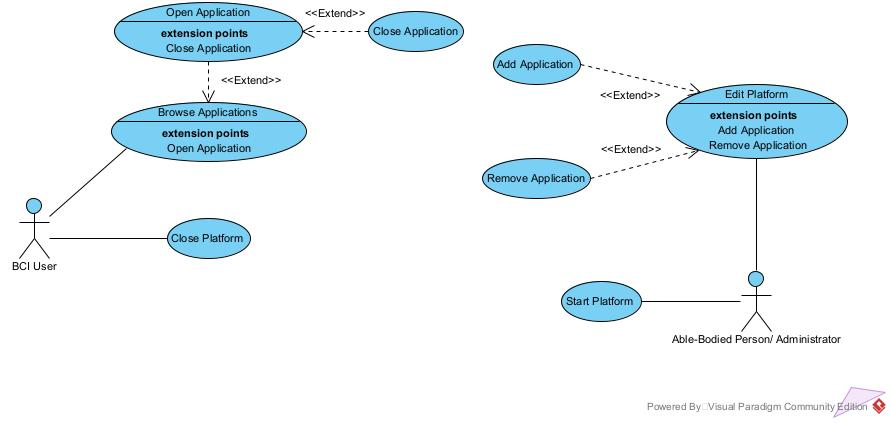
\includegraphics[width = 420pt]{Diagrams/Use Case.jpg}

\hspace{\parindent} The app will primarily be used by 2 categories of users: BCI users and able-bodied users/app administrators. BCI users will be the actual users of the app while the administrators' role will be maintenance or starting the application. 

\hspace{\parindent} The BCI users can use the platform through the brain computer interface. They can choose from a selection of different applications using a intuitive graphical user interface provided by the platform. Once selected, the application may be used indefinitely or until the user decides he/she is done with it, at which point the app may be closed by the users, bringing them back to the main page of the platform. Alongside using the applications, the user may also close the platform altogether. In the case of patients that cannot talk, this can be useful to signal a caretaker that they are done for the day.

\hspace{\parindent} The app administrator or generally any able-bodied person with knowledge of the platform can edit the apps housed by said platform at any time, adding or removing applications accordingly. They may also start the platform, since a BCI user without motor skills cannot do this by their own volition.


%%%%%%%%%%%% Section: Architectural Schematic %%%%%%%%%%%%
\subsection{Architectural Schematic}\label{subsect:architectural schematic}
\vspace{20pt}
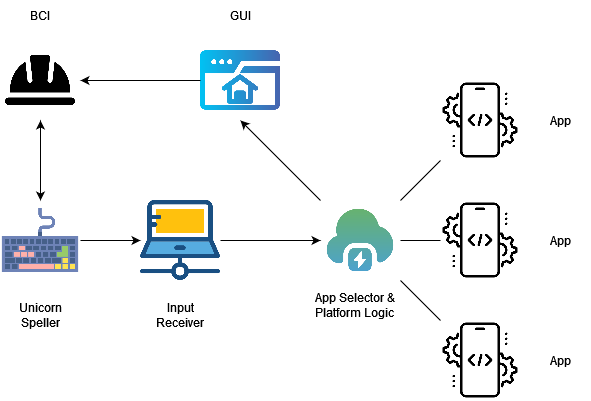
\includegraphics[width = 420pt]{Diagrams/Architectural.png}

\vspace{5pt}
\noindent {\tiny Icons courtesy of: Ayub Irawan, Flat Icons, Graphic's Plazza, iconmas, Kalashnyk, Prosymbols \cite{Cool_Icons}}
\vspace{25pt}

\hspace{\parindent} The main point of the app architecture is the Brain Computer interface itself. Through it the user can communicate with the Unicorn Speller, the proprietary software created by Unicorn to allow disabled people to communicate. Using the same software and a receiver we can take signals from the users and process them as actions inside the platform. At which point the platform makes the necessary changes to the GUI that the user sees and communicates accordingly with one of the applications housed in the platform, if the user selected one.


%%%%%%%%%%%%%%%%%%%%%%%%%%%%%%%%%%%%%%%%%%%%%%%%%%%%
%%%%%%%%%%%% Section: Similar Solutions %%%%%%%%%%%%
%%%%%%%%%%%%%%%%%%%%%%%%%%%%%%%%%%%%%%%%%%%%%%%%%%%%%%%%%%%%%%%%%%%%%%%%%%%%%%%%%%%%%%%%%%%%%%%%%%%%%%%%%%%%%%%%%%%%%%%%%%%%%%%%%%%%%%%%%%%%%%%%%%%%%%%%%%%%
\section{Similar Solutions}\label{sect:similar solutions}
\hspace{\parindent} Since the field of Brain Computer interfacing is still in its infancy, not many similar solutions exist, at least in the public space. There are multiple suites of applications available on the market, including the proprietary software Unicorn uses alongside their hardware which will also be used to build this application. All these software solutions require an able-bodied person to step in to change between applications, boards and at times even recalibrate the BCI hardware however. Thus, at the time of writing this paper, no similar solutions are known.

\hspace{\parindent} Disclaimer: While at the time of writing I am not aware of any similar solutions, this is subject to change as I further research this subject. Thereupon, as long as this paper is being redacted, I will update this section accordingly. {\bfseries(TODO: MOVE SECTION)}
